\documentclass{article}

\usepackage{fancyhdr}
\usepackage{extramarks}
\usepackage{amsmath}
\usepackage{amsthm}
\usepackage{amsfonts}
\usepackage{tikz}
\usepackage[plain]{algorithm}
\usepackage{algpseudocode}
\usepackage{graphicx}
\usepackage{gensymb}
\usepackage{calc}
\usepackage[framed,numbered,autolinebreaks,useliterate]{mcode}
\usepackage{listings}
\usepackage{empheq}
\usepackage{enumitem}
\usepackage[font=footnotesize]{caption}

\graphicspath{{./images/}}

\usetikzlibrary{automata,positioning}

%
% Basic Document Settings
%

\topmargin=-0.45in
\evensidemargin=0in
\oddsidemargin=0in
\textwidth=6.5in
\textheight=9.0in
\headsep=0.25in

\linespread{1.1}

\pagestyle{fancy}
\lhead{\hmwkAuthorLastNames}
\chead{\hmwkClass\ \hmwkTitle}
\rhead{\firstxmark}
\lfoot{\lastxmark}
\cfoot{\thepage}

\renewcommand\headrulewidth{0.4pt}
\renewcommand\footrulewidth{0.4pt}

\setlength\parindent{0pt}

%
% Create Problem Sections
%

\newcommand{\enterProblemHeader}[1]{
    \nobreak\extramarks{}{Problem {#1} continued on next page\ldots}\nobreak{}
    \nobreak\extramarks{{#1} (continued)}{{#1} continued on next page\ldots}\nobreak{}
}

\newcommand{\exitProblemHeader}[1]{
    \nobreak\extramarks{{#1} (continued)}{{#1} continued on next page\ldots}\nobreak{}
    % \stepcounter{#1}
    \nobreak\extramarks{{#1}}{}\nobreak{}
}

\setcounter{secnumdepth}{0}
\newcounter{partCounter}

\newcommand{\problemNumber}{0.0}

\newenvironment{homeworkProblem}[1][-1]{
    \renewcommand{\problemNumber}{{#1}}
    \section{\problemNumber}
    \setcounter{partCounter}{1}
    \enterProblemHeader{\problemNumber}
}{
    \exitProblemHeader{\problemNumber}
}

%
% Homework Details
%   - Title
%   - Class
%   - Author
%

\newcommand{\hmwkTitle}{Group Assignment\ \#1}
\newcommand{\hmwkClass}{RBE 500}
\newcommand{\hmwkAuthorName}{\textbf{Joshua Gross, Arjan Gupta, Melissa Kelly}}
\newcommand{\hmwkAuthorLastNames}{\textbf{Gross, Gupta, Kelly}}

%
% Title Page
%

\title{
    \vspace{2in}
    \textmd{\textbf{\hmwkClass\ \hmwkTitle}}\\
    \vspace{3in}
}

\author{\hmwkAuthorName}
\date{}

\renewcommand{\part}[1]{\textbf{\large Part \Alph{partCounter}}\stepcounter{partCounter}\\}

%
% Various Helper Commands
%

% Useful for algorithms
\newcommand{\alg}[1]{\textsc{\bfseries \footnotesize #1}}

% For derivatives
\newcommand{\deriv}[2]{\frac{\mathrm{d}}{\mathrm{d}#2} \left(#1\right)}

% For compact derivatives
\newcommand{\derivcomp}[2]{\frac{\mathrm{d}#1}{\mathrm{d}#2}}

% For partial derivatives
\newcommand{\pderiv}[2]{\frac{\partial}{\partial #2} \left(#1\right)}

% For compact partial derivatives
\newcommand{\pderivcomp}[2]{\frac{\partial #1}{\partial #2}}

% Integral dx
\newcommand{\dx}{\mathrm{d}x}

% Alias for the Solution section header
\newcommand{\solution}{\textbf{\large Solution}}

% Probability commands: Expectation, Variance, Covariance, Bias
\newcommand{\E}{\mathrm{E}}
\newcommand{\Var}{\mathrm{Var}}
\newcommand{\Cov}{\mathrm{Cov}}
\newcommand{\Bias}{\mathrm{Bias}}

\newlength\dlf% Define a new measure, dlf
\newcommand\alignedbox[2]{
% Argument #1 = before & if there were no box (lhs)
% Argument #2 = after & if there were no box (rhs)
&  % Alignment sign of the line
{
\settowidth\dlf{$\displaystyle #1$}  
    % The width of \dlf is the width of the lhs, with a displaystyle font
\addtolength\dlf{\fboxsep+\fboxrule}  
    % Add to it the distance to the box, and the width of the line of the box
\hspace{-\dlf}  
    % Move everything dlf units to the left, so that & #1 #2 is aligned under #1 & #2
\boxed{#1 #2}
    % Put a box around lhs and rhs
}
}

\begin{document}

\maketitle

\nobreak\extramarks{Problem 1}{}\nobreak{}

\pagebreak

\begin{homeworkProblem}[Problem 1]
    \subsection{Create SCARA Robot in Gazebo}

    The 3 DOF SCARA robot we have built is shown below.

    \begin{figure}[h]
        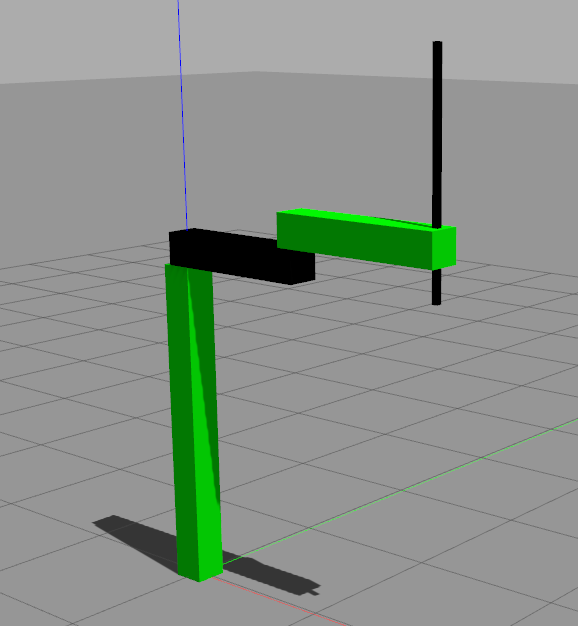
\includegraphics[scale=0.47]{gazebo-final-scara.png}
        \centering
    \end{figure}

    We undertook the following steps to create our SCARA robot.

    \subsubsection{1 --- Modify joint locations}

    In the downloaded package, the RRBot robot has its revolute joints on the `sides' of its links, as shown in the following figure.
    
    \begin{figure}[h]
        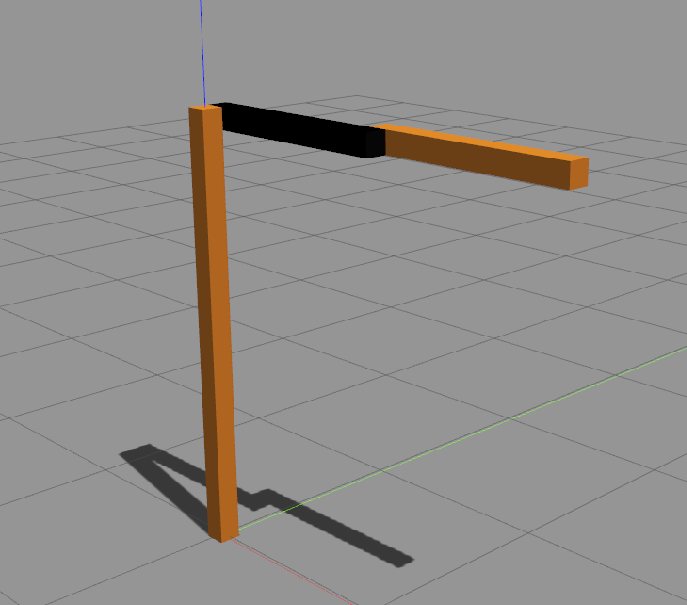
\includegraphics[scale=0.25]{initial-rrbot.png}
        \centering
    \end{figure}

    However, for a standard SCARA robot, we want the revolute joints to sweep angles in the XY plane of the world frame, not in the XZ plane.
    
    Hence, we edited the \lstinline{<joint>} element blocks in the URDF file rrbot\_description.urdf.xacro. For the first joint, we made the following
    change.

    \lstinputlisting[language=XML, firstline=51,lastline=59]{../ros2-code/src/rrbot_simulation_files/rrbot_description/urdf/rrbot_description.urdf.xacro}
    \vspace{0.15in}

    In the above code snippet, we changed the type attribute of the joint element from continuous to revolute. We also added the limit sub-element, and
    modified the origin and axis sub-elements. We made similar changes for the second joint, for which the code snippet is shown below.

    \lstinputlisting[language=XML, firstline=87,lastline=95]{../ros2-code/src/rrbot_simulation_files/rrbot_description/urdf/rrbot_description.urdf.xacro}
    \vspace{0.15in}

    As a result, our robot now looked like the following image.

    \begin{figure}[h]
        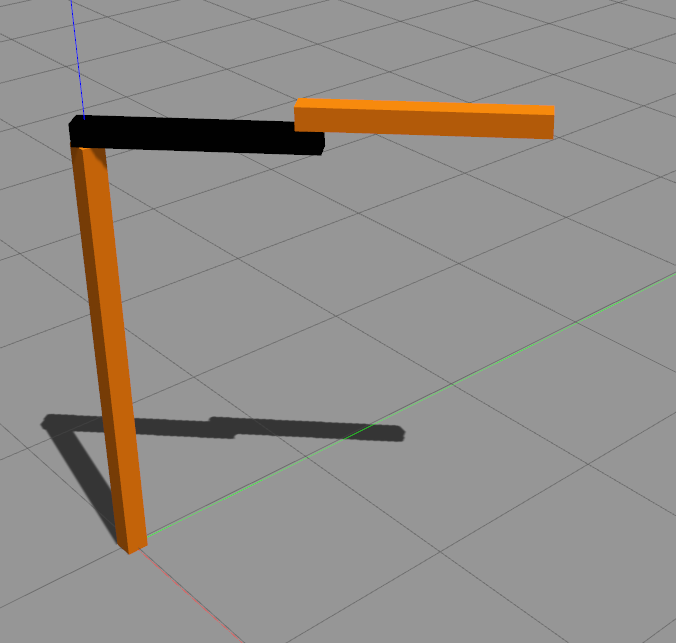
\includegraphics[scale=0.25]{top-joints-rrbot.png}
        \centering
    \end{figure}

    In order to test our changes, we moved our robot by publishing joint values in the format of the following ROS command in our terminal.

    \begin{lstlisting}
        ros2 topic pub --once /forward_position_controller/commands std_msgs/msg/Float64MultiArray "{data: [0.75 0.82]}"
    \end{lstlisting}

    \subsubsection{2 --- Add prismatic joint}

    Now our revolute joints resemble those of a SCARA robot, but we still need a prismatic joint. In order to do this, we first made the following
    changes to the rrbot\_description.urdf.xacro file.

    \lstinputlisting[language=XML, firstline=123,lastline=158]{../ros2-code/src/rrbot_simulation_files/rrbot_description/urdf/rrbot_description.urdf.xacro}
    \vspace{0.15in}

    In the above code snippet, we have changed the tool joint from fixed to prismatic, defined its translation axis, set its limits, and defined its origin.
    We defined a special \lstinline{prismatic_width} so that we could make the tool link thinner than the regular links. We also defined a
    \lstinline{prismatic_offset} so that the tool link is slightly `lowered'. This makes it so that the zero position of the tool link is at the
    same height as our first link, which makes our calculations consistent with our forward-kinematics derivation.\\

    Next, we defined the tool joint in the rrbot.ros2\_control.xacro file, so that the command and state interfaces for ROS2 could be made available 
    for that joint. Finally, we also edited the gazebo\_controllers.yaml file to define the tool joint as part of the three
    controllers --- \lstinline{forward_position_controller}, 
    \lstinline{forward_velocity_controller}, and \lstinline{forward_effort_controller}. All these modified files have been included as part of our submission
    inside the rrbot\_description.zip compressed directory.

    At this point, our robot looked as follows.
    
    \begin{figure}[h]
        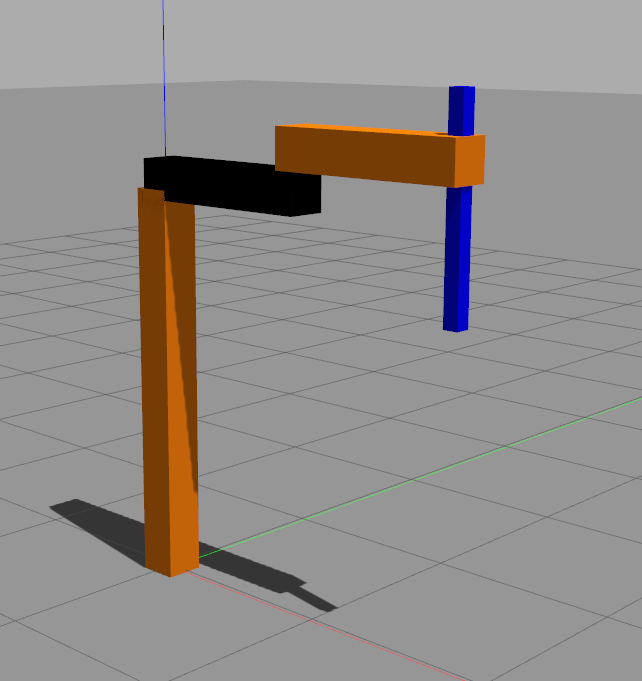
\includegraphics[scale=0.25]{unfinished-scara.png}
        \centering
    \end{figure}

    After this, we tweaked some offsets, adjusted some link lengths, changed the colors of the robot, and decreased the thickness of the tool link in order
    to arrive at our finished implementation of the SCARA robot. We also used the same ROS command as earlier (except with 3 data-points this time) to ensure
    that we were able to move all the joints of our robot.

\end{homeworkProblem}

\nobreak\extramarks{Question 2}{}\nobreak{}

\begin{homeworkProblem}[Question 2]
    \subsection{Forward Kinematics for SCARA}

    Before implementing forward kinematics in ROS, we worked out a derivation for the forward kinematics of the SCARA robot model.

    \subsubsection{Derviation}

    The image below shows the frame assignments for the robot.
    
    \begin{figure}[h]
        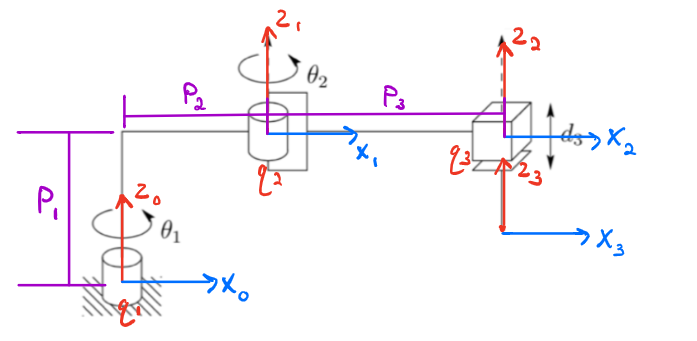
\includegraphics[scale=0.55]{fwd-kin-frames-whitebg.png}
        \centering
    \end{figure}

    Based on this, we can form the DH table as shown on the next page.
    
    \vspace{3in}
    
    \begin{table}[h!]
        \begin{center}
            \begin{tabular}{|c|c|c|c|c|}
            \hline
            Link & $\alpha_i$ & $a_i$ & $\theta_i$ & $d_i$ \\
            \hline
            1 & 0 & $p_2$ & $q_1$ & $p_1$ \\
            2 & 0 & $p_3$ & $q_2$ & 0\\
            3 & 0 & 0 & 0 & $q_3$ \\
            \hline
            \end{tabular}
        \end{center}
    \end{table}

    Next, we create a MATLAB script as shown below. We use the matrix obtained from equation 3.10 of the textbook to write \(A_1, A_2, A_3\). By multiplying 
    these matrices, we obtain the $T^0_3$.

    \lstinputlisting[language=MATLAB]{Project_Part1_fk.m}

    This MATLAB script gives us the following $T^0_3$ matrix, which is the homogeneous transformation for the end-effector with respect to the base frame. 

    \[
        \begin{bmatrix}\cos{q_1}\,\cos{q_2}-\sin{q_1}\,\sin{q_2} & -\cos{q_1}\,\sin{q_2}-\cos{q_2}\,\sin{q_1} & 0 & P_{2}\,\cos{q_1}+P_{3}\,\cos{q_1}\,\cos{q_2}-P_{3}\,\sin{q_1}\,\sin{q_2}\\ \cos{q_1}\,\sin{q_2}+\cos{q_2}\,\sin{q_1} & \cos{q_1}\,\cos{q_2}-\sin{q_1}\,\sin{q_2} & 0 & P_{2}\,\sin{q_1}+P_{3}\,\cos{q_1}\,\sin{q_2}+P_{3}\,\cos{q_2}\,\sin{q_1}\\ 0 & 0 & 1 & P_{1}+q_{3}\\ 0 & 0 & 0 & 1 \end{bmatrix}
    \]

    \subsubsection{ROS Implementation of Forward Kinematics}

    For implementing the ROS portion of forward kinematics, we lorem ipsum dolor sit amet, consectetur adipiscing elit, sed do eiusmod tempor incididunt ut labore et dolore magna aliqua. Purus semper eget duis at tellus at. Ac turpis egestas integer eget aliquet nibh. Aliquam etiam erat velit scelerisque in. Ac turpis egestas sed tempus urna et pharetra pharetra. Faucibus in ornare quam viverra. Libero id faucibus nisl tincidunt eget.\\
    
    Aenean pharetra magna ac placerat vestibulum lectus mauris. Consequat nisl vel pretium lectus quam id leo. Lorem sed risus ultricies tristique nulla aliquet enim tortor at. Ligula ullamcorper malesuada proin libero nunc.

    \subsubsection{Gazebo Screenshots with ROS Output}

    \underline{Pose 1}

    Below are screenshots for joint values $q_1 = 30\degree$, $q_2 = 47\degree$, $q_3 = 0.7$

    \vspace{7in}

    \underline{Pose 2}

    Below are screenshots for joint values $q_1 = 72\degree$, $q_2 = 28\degree$, $q_3 = 1.05$

    \vspace{5in}

    \underline{Pose 3}

    Below are screenshots for joint values $q_1 = 72\degree$, $q_2 = 28\degree$, $q_3 = 1.05$

    \vspace{3in}

\end{homeworkProblem}

\nobreak\extramarks{Question 3}{}\nobreak{}

\begin{homeworkProblem}[Question 3]
    \subsection{Inverse Kinematics for SCARA}
\end{homeworkProblem}

\end{document}